\documentclass[11pt, oneside]{article}   	% use "amsart" instead of "article" for AMSLaTeX format
\usepackage{geometry}                		% See geometry.pdf to learn the layout options. There are lots.
\geometry{letterpaper}                   		% ... or a4paper or a5paper or ... 
%\geometry{landscape}                		% Activate for rotated page geometry
%\usepackage[parfill]{parskip}    		% Activate to begin paragraphs with an empty line rather than an indent
\usepackage{graphicx}				% Use pdf, png, jpg, or eps§ with pdflatex; use eps in DVI mode
								% TeX will automatically convert eps --> pdf in pdflatex		
\usepackage{amssymb}

%SetFonts
\graphicspath{ {./images/} } 				

%SetFonts


\title{Algoritmi e Strutture dati}
\author{Federico Zhou}
%\date{}							% Activate to display a given date or no date

\begin{document}
\maketitle
\section{Introduzione e motivazioni}
Un algoritmo è un insieme ordinato e finito di passi eseguibili non ambigui che definiscono un procedimento che termina. Le operazioni di analisi sugli algoritmi sono basati sull'analisi di \emph{correttezza, complessità, efficienza}, basate sul \emph{tempo, spazio, costo}.\\
Per analizzare gli algoritmi utilizziamo le notazioni asintotiche, che sono: $O$, $\Omega$ e $\Theta$.\\
I parametri su cui facciamo le analisi sono:
\begin{itemize}
\item Complessità in tempo: tempo richiesto per terminare l'esecuzione
\item Complessità in spazio: quantità di spazio richiesto per terminare l'esecuzione.
\end{itemize}
Dobbiamo tuttavia parlare prima del modello di calcolo: quando facciamo l'analisi del tempo e dello spazio, possiamo farlo contando la singola operazione come un singolo passo, indipendentemente dalla dimensione degli operandi. Questo tuttavia è irrealistico, l'algoritmo che calcola fibonacci cresce in maniera esponenziale. Per ovviare a questo problema è stato introdotto il modello di calcolo del costo logaritmico che assume che il costo di esecuzione delle istruzioni dipenda dalla dimensione degli operandi coinvolti.
\begin{itemize}
\item Criterio del costo uniforme\\
- Tempo: ogni istruzione utilizza un'unità di tempo indipendentemente dalla grandezza degli operandi
- Spazio: ogni variabile utilizza un'unità di spazio indipendentemente dalla grandezza del valore
\item Criterio del costo logaritmico\\
- Tempo: ogni operazione utilizza un tempo proporzionale alla lunghezza dei valori 
- Spazio: ogni variabile utilizza un'unità di spazio dipendente dalla rappresentazione del dato
\end{itemize}
Gli algoritmi con cui lavoriamo possono avere tempo:
\begin{itemize}
\item polinomiale, algoritmi che lavorano in un tempo limitato da un polinomio, ragionevoli e praticabili
\item esponenziali, algoritmi che lavorano in tempo esponenziale, non praticabili.
\end{itemize}
\section{Algoritmi di ordinamento}
Gli algoritmi di ordinamento sono tantissimi, ma si possono suddividere principalmente in 2 categorie: ad ordinamento interno se l'ordinamento avviene su dati in memoria centrale, e a ordinamento esterno se l'ordinamento avviene su dati in memoria di massa.\\
Gli algoritmi di ordinamento che analizziamo noi vengono applicati su array:
\begin{itemize}
\item gli array sono strutture di dati statiche, con elementi omogenei
\item gli elementi in un array sono salvati consecutivamente, e sono individuati in base alla loro posizione rispetto al primo elemento.
\item l'accesso in un array è diretto, l'operazione di lettura e modifica ha complessità $O(1)$
\end{itemize}
Gli algoritmi che studieremo si basano sul confronto di chiavi, in quanto è l'operazione più costosa. Studieremo lo spazio: la memoria occupata nello stack, ed il tempo: la complessità di tempo\\\\
\textbf{Stabilità in un algoritmo:}\\
Un algoritmo è detto stabile se preserva l'ordine relativo tra i record con medesima chiave. I record che hanno una stessa chiave vengono lasciati nell'ordine originale.\\
\textbf{Operabilità "sul posto":}\\
Quando parliamo di un algoritmo che "opera sul posto" parliamo di un algoritmo che non ha bisogno di una struttura d'appoggio. Alcuni esempi sono il MergeSort, che utilizza un array d'appoggio
\subsection{Algoritmi elementari}
In particolare gli algoritmi elementari sono SelectionSort, InsertionSort, BubbleSort, sono algoritmi che utilizzano $\Theta(n^2)$ confronti.
Iniziamo da SelectionSort e InsertionSort dato che lavorano in maniera simile:\\
- all'inizio di ciascun passo l'array contiene una parte ordinata, ed una parte da ordinare\\
- alla fine del passo il segmento ordinato contiene un elemento in più, alla fine dei passi totali l'array è ordinato.
\begin{itemize}
\item SelectionSort\\
Cerco l'elemento più piccolo nella porzione non ordinata e lo metto in coda alla porzione ordinata. L'indicatore della porzione ordinata avanza di uno, per $n-1$ volte.
\begin{center}
\includegraphics[scale=0.8]{selSort}
\end{center}
SelectionSort è un algoritmo stabile (perché utilizza \textless al posto di \textless=, la sua complessità in tempo è la medesima sia nel caso peggiore che ne caso peggiore, ovvero $\Theta(n^2)$
\item InsertionSort\\
Prendo un elemento nella parte non ordinata e lo inserisco nella posizione giusta all'interno della parte ordinata. Sposto di avanti un indice la parte ordinata.
\begin{center}
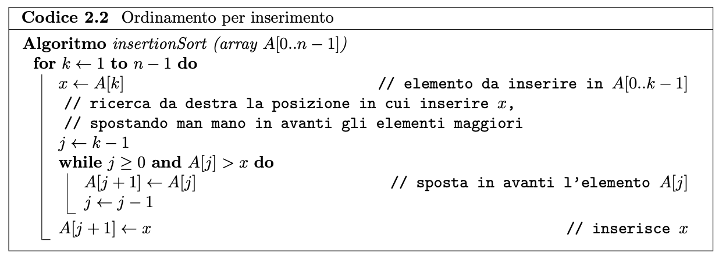
\includegraphics[scale=0.8]{insort}
\end{center}
InsertionSort è un algoritmo stabile, nel caso peggiore la complessità di tempo è $\Theta(n^2)$ ma nel caso migliore il numero di confronti da fare è $n-1$
\item BubbleSort\\
Scansiona l'array e confronto coppie adiacenti ripetutamente, scambio gli elementi se sono in ordine diverso. Alla fine dell'ultimo round l'elemento più grande finisce sul fondo.
\begin{center}
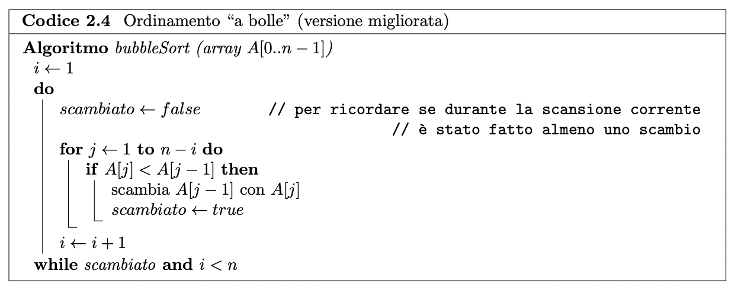
\includegraphics[scale=0.8]{bubsort}
\end{center}
BubbleSort è un algoritmo stabile, nel caso peggiore la complessità di tempo è $\Theta(n^2)$ ma nel caso migliore il numero di confronti da fare è $n-1$
\end{itemize}
\subsection{Algoritmi avanzati}
In particolare gli algoritmi avanzati sono MergeSort, QuickSort, HeapSort, sono algoritmi che utilizzano $\Theta(nlogn)$ confronti.
\begin{itemize}
\item MergeSort\\
Dividi l'array in porzioni unitarie, ordina ordina ricorsivamente le porzioni adiacenti fino a ricostruire l'array ordinato. 
\begin{center}
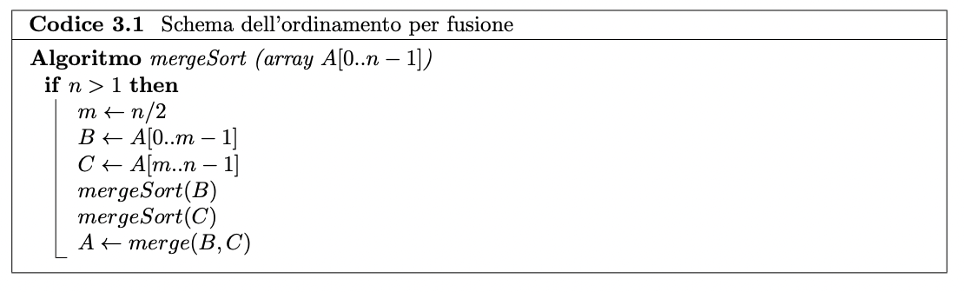
\includegraphics[scale=0.8]{mergsort}
\end{center}
MergeSort è un algoritmo stabile, non opera sul posto ed è più efficiente degli algoritmi visti in precedenza.\\ \\Per funzionare l'algoritmo MergeSort ha bisogno di un metodo che ci permetta di fare la fusione tra 2 array, in particolare dati due array $B, C$ dobbiamo avere un array $A$ che sia uguale all'unione tra $B, C$.\begin{center}
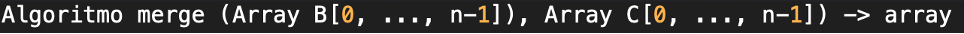
\includegraphics[scale=0.8]{merge}
\end{center}
\item QuickSort\\
1. Scegli un elemento n di A come perno\\
2. Inserisci tutti gli elementi $n \leq a$ in un array B\\
3. Inserisci tutti gli elementi $n > a$ in un array C\\
4. Ordina B e C\\
5. Unisci B e C
\begin{center}
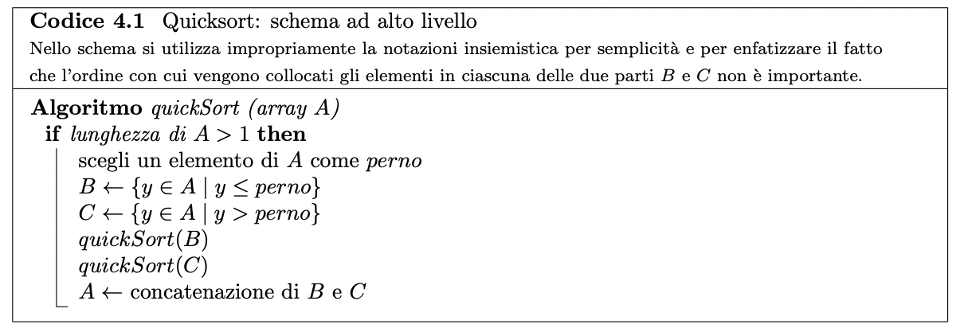
\includegraphics[scale=0.8]{quicksort}
\end{center}
QuickSort è il primo algoritmo instabile che incontriamo. Diversamente da MergeSort, QuickSort opera sul posto in quanto utilizzano soltanto due variabili aggiuntive. \\Nel caso ottimo l'algoritmo ha un tempo \begin{center} $T(n) = O(n * logn)$ \end{center}nel caso pessimo invece \begin{center} $T(n) = O(n^2)$ \end{center} Nel caso medio QuickSort opera in $T(n) = O(n * logn)$
In media QuickSort è più efficiente di InsertionSort, SelectSort, BubbleSort e ha prestazioni peggiori di MergeSort solo nel caso peggiore. Da verifiche sperimentali possiamo concludere che QuickSort è l'array più efficiente. Possiamo inoltre concludere che in genere $T(n) = O(n * logn)$ è il tempo migliore possibile per gli algoritmi di ordinamento basati sul confronto
\end{itemize}
\section{Tecniche di risoluzione}
\subsection{Tecniche Divide-Et-Impera}
La tecnica del divide et impera è una tecnica di progettazione degli algoritmi che consiste in 3 fasi:
\begin{itemize}
\item dividere l'istanza dei dati in ingresso in più sottoinstanze disgiunte
\item risolvere ricorsivamente i problemi in ciascuna sottoistanza separatamente
\item combinare le soluzioni delle sottoinstanze per ricavare la soluzione dell'istanza iniziale.
\end{itemize}
L'efficienza del metodo dipende dal metodo di decomposizione e ricomposizione delle soluzioni parziali. Questa tecnica adotta un approccio top-down, i principali esempi che vediamo noi sono MergeSort e QuickSort. Una generalizzazione della tecnica può essere la seguente:
\begin{center}
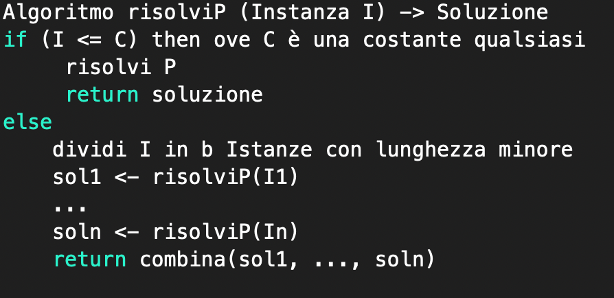
\includegraphics[scale=0.8]{divide}
\end{center}
Gli esempio che abbiamo visto durante il corso di applicazione di tecniche divide-et-impera sono:
\begin{itemize}
\item algoritmo ricorsivo per calcolare il massimo ed il minimo subarray di un array di $n$ interi\\
L'array iniziale è suddiviso in 3 subarray disgiunti di $n/2$ interi, e ricorsivamente calcoliamo il massimo o il minimo di ciascun subarray.
\item Algoritmo di ricerca binaria in un array di $n$ interi\\
L'algoritmo divide l'array in due subarray di grandezza $n/2$ ricorsivamente, procedendo solo in uno dei due subarray.
\item Mergesort per array di $n$ elementi\\
L'algoritmo divide l'array in due subarray di grandezza $n/2$ ricorsivamente, e riordina ciascuno dei subarray, riunendoli alla fine
\item Quicksort per array di $n$ elementi\\
L'algoritmo divide l'array in tre subarray disgiunti composti rispettivamente dagli elementi $\leq$, $=$ e $\geq$. Il primo ed il terzo array sono riordinati ricorsivamente, e vengono poi concatenati i subarrays. 
\end{itemize}
\subsection{Dynamic Programming | Programmazione dinamica}
La programmazione dinamica è una tecnica di progettazione di algoritmi che diversametne dal divide-et-impera opera secondo una logica bottom-up; la risoluzione si basa sulla risoluzione di sottoproblemi progressivamente più grandi. Ne consegue che per tenere conto delle soluzioni ai sottoproblemi la tecnica di programmazione dinamica utilizza un'apposita tabella.\\
Possiamo dividere la tecnica di programmazione dinamica in quattro fasi:
\begin{itemize}
\item Identificazione dei sottoproblemi del problema iniziale
\item Predisporre una tabella ove memorizzare dinamicamente le soluzioni ai sottoproblemi a partire dai sottoproblemi più semplici
\item Si utilizzano le soluzioni dei sottoproblemi precedentemente risolti per risolvere sottoproblemi più difficili
\item Si costruisce la soluzione finale a partire dalle soluzioni dei sottoproblemi risolti.
\end{itemize}
La programmazione dinamica, come negli algoritmi greedy, rappresentano problemi di ottimizzazione e seguono il principio di ottimalità, che garantisce che se una soluzione è ottima, anche le porzioni che vanno a comporre la situazione sono ottime
Gli esempio che abbiamo visto durante il corso di applicazione di tecniche programmazione dinamica sono:
\begin{itemize}
\item L'algoritmo di Floyd-Warshall per un grafo di $n$ vertici.
Identifica come sottoproblemi quelli di calcolare i percorsi più brevi tra tutte le coppie di vertici del grafo che passano per vertici di indice $\leq$ $k$ per ogni $1 \leq k$ $<$ $n$, predispone una tabella di $n + 1$ elementi (che sono delle matrici quadrate di ordine $n$) inizializzando il primo elemento in base alla matrice di adiacenza del grafo, avanza di un elemento alla volta determinandone il valore tramite una specifica formula applicata al valore dell’elemento precedente, e restituisce come risultato il valore dell’ultimo elemento. In pratica, non serve predisporre una tabella di matrici in quanto è sufficiente un’unica matrice per effettuare tutti i calcoli.
\end{itemize}
\subsection{Greedy Algorithms | Tecnica golosa}
La tecnica golosa si applica ai problemi di ottimizzazione in cui la soluzione è costruita scegliendo, ad ogni passo, l'elemento migliore nel momento. La soluzione che ricaviamo non è sempre la soluzione ottima, è tuttavia la soluzione più veloce da computare
Gli esempio che abbiamo visto durante il corso di applicazione di tecniche greedy sono:
\begin{itemize}
\item Algoritmo di Kruskal per grafo ricoprente minimo\\
L'algoritmo di Kruskal costruisce la soluzione considerando come candidati i singoli archi del grafo, scegliendo ad ogni passo l'arco di peso minimo tra i rimasti, ritenendo i singoli archi ammissibili se i vertici appartengono a due alberi diversi tra quelli costruiti fino a quel momento
\item Algoritmo di Prim per grafo ricoprente minimo\\
L'algoritmo di Prim costruisce la soluzione partendo da un grafo iniziale contentente un solo vertice $s$, considerando come candidati i rimanenti vertici del grafo scegliendo ad ogni passo quelli con distanza minima dall'albero libero costruito fino a quel momenti.
\item Algoritmo di Dijkstra per il calcolo di cammino minimo tra un vertice $s$ e tutti gli altri\\
L'algoritmo prende come soluzione iniziale un insieme vuoto (con input iniziale un vertice $s$), considerando come candidati i singoli vertici del grafo, scegliendo tra quelli rimasti quelli con distanza minima dal vertice sorgente.
\end{itemize}




\section{Tipi di dati}
Il tipo di una variabile rappresenta una variabile che stabilisce i valori che il dato può assumere e le operazioni che essa può svolgere. Le varie strutture dati che andiamo ad analizzare sono riconducibili a quattro classi fondamentali, ovvero: \emph{array, liste, alberi e grafi.} Le strutture dati possono essere caratterizzate dalla loro occupazione di memoria, che può essere statica, o dinamica.

\subsection{Dizionario | HashMap}
Il dizionario è una collezione di elementi ciascuno dei quali è caratterizzato da una \textbf{chiave}. Le operazioni che possiamo svolgere su un dizionario sono \emph{la ricerca, l'inserimento e la cancellazione} di un elemento. \\
Un dizionario può essere implementato utilizzando un array:\\
- se l'array è ordinato in base la chiave la ricerca ha costo $\Theta(logn)$ e l'inserimento costa $\Theta(n)$
- se l'array invece non è ordinato la ricerca costa $\Theta(n)$ e l'inserimento costa $\Theta(1)$\\\\
Un dizionario può essere anche implementato utilizzando collezioni, ovvero strutture statiche (con dimensione fissata all'inizializzazione), indicizzate ad esempio \emph{vectors e arraylists}; oppure utilizzando strutture collegate, dinamiche ad esempio \emph{liste e alberi}

\subsection{Liste concatenate}
Le liste concatenate sono un insieme di nodi collegati linearmente tra di loro. In particolare ogni nodo contiene:
\begin{itemize}
\item un dato della collezione
\item informazioni per accedere al prossimo nodo
\item informazioni per accedere al nodo precedente (nel caso delle doppiamente concatenate)
\end{itemize}
\begin{center}
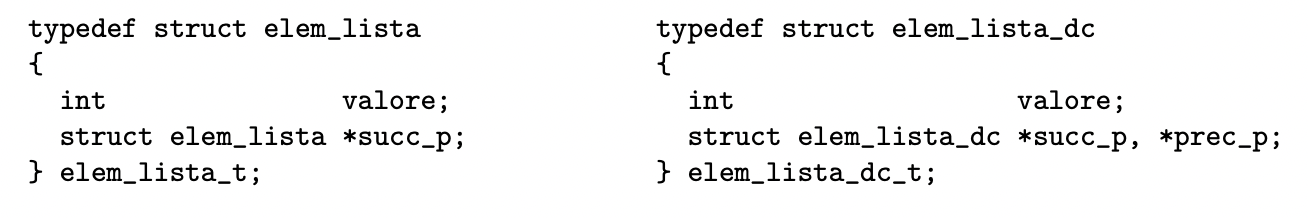
\includegraphics[scale=0.7]{conca}
\end{center}
I tipi di problemi che possiamo andare a svolgere sulle liste sono:
\begin{itemize}
\item problema della visita: data una lista attraversare tutti gli elementi una volta
\item problema della ricerca, data una lista ed un valore, stabilire se il valore è contenuto all'interno della lista, e l'indirizzo in caso affermativo
\item problema dell'inserimento, data una lista ed un valore, inserire il valore nella posizione appropriata
\item problema della rimozione, data una lista ed un valore, rimuovere il valore dalla lista
\end{itemize}

\subsection{Pila}
La pila, o stack, è una struttura dati che organizza i dati secondo una logica LIFO, il che significa che gli inserimenti e le rimozioni avvengono presso l'estremità della lista. Come in una lista la pila è individuata dall'indirizzo per primo elemento, chiamato cima. L'implementazione può avvenire con un array, o delle liste lineari. Le operazioni fondamentali che vengono svolte su una pila sono:
\begin{itemize}
\item isEmpty: che mi restituisce true se la pila è vuota, e false se la pila non lo è
\item push: dato un valore, lo aggiunge sulla pila
\item pop: dato un valore, lo rimuove dalla pila
\item peek: mi restituisce il valore in cima, senza modificarla
\end{itemize}

\subsection{Alberi con radice}
Gli alberi con radice (o solamenta albero) sono una struttura dati simile agli array, ma dotati di una rappresentazione gerarchica dei dati. I nodi possono essere definiti come padre, nodo interno, foglia e radice, mentre i collegamenti tra i nodi sono chiamati archi. In particolare quando parliamo di alberi possiamo identificare:
\begin{itemize}
\item la profondità come il numero massimo di nod da attraversare partendo dalla radice alla foglia più distante
\item grado di un nodo come il numero massimo di figli che un nodo può avere
\end{itemize}
I problemi classici che trattiamo per gli alberi sono: visita, ricerca, inserimento e rimozione. 
\subsubsection{Alberi binari}
Un albero è detto binario se ad ogni nodo sono associati al più 2 figli, chiamati rispettivamente figlio destro e figlio sinistro. 
\subsubsection{Alberi binari di ricerca}
Un albero è detto binario di ricerca se:
\begin{itemize}
\item tutti gli elementi nel sottoalbero sinistro hanno valore $<$ della chiave in $n$
\item tutti gli elementi nel sottoalbero destro hanno valore $\geq$ della chiave in $n$
\end{itemize}
Gli alberi binari di ricerca differiscono dagli alberi binari in quanto permettono una \emph{ricerca più efficiente} degli alberi binari. In particolare per ogni nodo incontrato si verifica se il valore si maggior o minore della chiave contenuta nel nodo. \\
L'inserimento e la rimozione devono invece garantire che l'albero binario risultante sia ancora un albero binario di ricerca.\\ La complessità degli algoritmi di ricerca, inserimento e rimozione con $n$ il numero di nodi, e $h$ la sua altezza:
\begin{center}
Caso ottimo: $T(n) = O(1)$\\
Caso pessimo: $T(n) = O(n)$\\
Caso medio: $T(n) = (log$ $n)$
\end{center}
\subsubsection{Alberi perfettamente bilanciati}
Un albero binario è detto perfettamente bilanciato se, per ogni nodo, il numero di nodi del suo sottoalbero sinistro, ed il numero di nodi del suo sottoalbero destro differiscono al più di 1.\\
\emph{Brutalmente: guardando sotto ogni sotto-nodo, la differenza tra il numero di nodi destro e sinistro è al massimo 1}\\
Siccome negli alberi perfettamente bilanciati, il bilanciamento dopo le operazioni di inserimento e rimozione sono costose sono stati introdotti una serie di alberi con forme di bilanciamento meno restrittive di quello perfetto.
\subsubsection{Alberi di ricerca AVL | Alberi bilanciati in altezza}
Un albero binario è detto bilanciato in altezza o AVL se, per ogni nodo, l'altezza del suo sottoalbero sinistro e l'altezza del suo sottoalbero destro differiscono al più di 1. Si noti che un albero perfettamente bilanciato anche bilanciato.
Gli alberi AVL sono particolari in quanto hanno un tempo di ricerca, inserimento e cancellazione pari che lavorano a tempo logaritmico:
\begin{center}
Per ricerca, inserimento e cancellazione:\\
$T(n) = O(log$ $n)$
\end{center}
\subsubsection{Alberi binario di ricerca rosso-nero}
Un albero binario di ricerca è detto rosso-nero se, dopo aver aggiunto un nodo sentinella come figlio di tutte le foglie, e dopo aver colorato ogni nodo di rosso o nero si ha che:
\begin{enumerate}
\item La radice è nera
\item La sentinella è nera
\item Se un nodo è rosso, tutti i suoi figli sono neri
\item per ogni nodo, tutti i percorsi dal nodo alla sentinella attraversano lo stesso numero di nodi neri
\end{enumerate}
Un albero binario di ricerca rosso-nero è una buona approssimazione di un albero binario di ricerca perfettamente bilanciato. 
\begin{center}
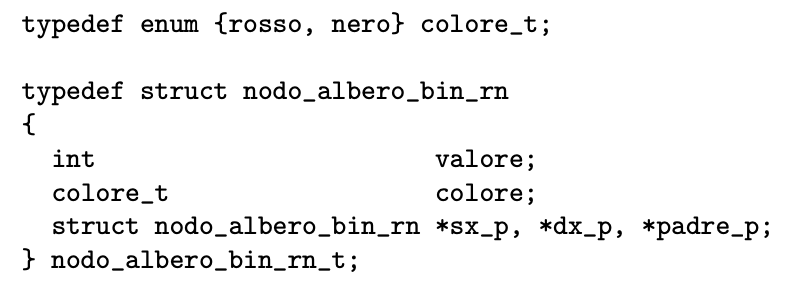
\includegraphics[scale=0.8]{rossonero}
\end{center}
\subsubsection{Alberi 2-3}
Un albero è detto 2-3 se ogni nodo interni ha 2-3 figli, e le foglie sono tutte allo stesso livello. I dati vengono inseriti all'interno delle foglie, mentre i nodi interni contengono solo informazioni di instradamento.\begin{itemize}
\item Se il nodo interno ha 1 valore, esso compare come sottofiglio sinistro, ed il sottofiglio destro è maggiore
\item Se il nodo interno ha 2 valori i sottofigli sono 3, i due valori compaiono come sottofiglio sinistro e centrale, mentre il sottofiglio destro è maggiore
\end{itemize}
\subsubsection{B-albero}
I B-alberi sono nati per rappresentare gli indici nelle basi di dati, l'obbiettivo è quello di minimizzare il numero di accessi. Le informazioni, a differenza degli alberi 2-3, sono presenti anche nei nodi interni.
Dato un b-albero di ordine $t$:
\begin{itemize}
\item i nodi interni hanno al massimo $2t$ figli
\item ogni nodo interno diverso dalla radice ha almeno $t$ figli
\item la radice ha almeno 2 figli
\item ogni foglia contiene $k$ chiavi ordinate
\end{itemize}
\begin{center}
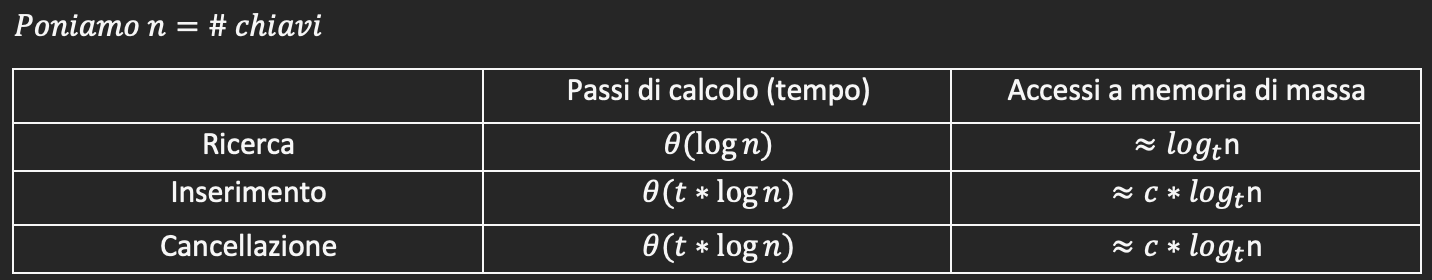
\includegraphics[scale=0.6]{balberi}
\end{center}
\subsubsection{Alberi binari quasi completi}
Un albero binario è detto \emph{quasi completo} quando è completo fino al penultimo livello e quindi tutte le foglie si trovano all'ultimo o penultimo livello.
\section{Heap}
Lo heap è un albero binario quasi completo, in cui la chiave contenuta in ciascun nodo è maggiore o uguale alle chiavi contenute nei figli. In particolare:
\begin{itemize}
\item tutte le foglie si trovano all'ultimo o penultimo livello
\item per ogni nodo, la chiave è $\geq$ delle chiavi contenute nei figli
\end{itemize}
\subsection*{Procedura risistema}
Consideriamo uno heap, se estraiamo un elemento è possibile sia necessario una \emph{risistemazione} dell'albero, in quanto potrebbe perdere la proprietà di heap. Questa procedura è implementata come segue:
\begin{center}
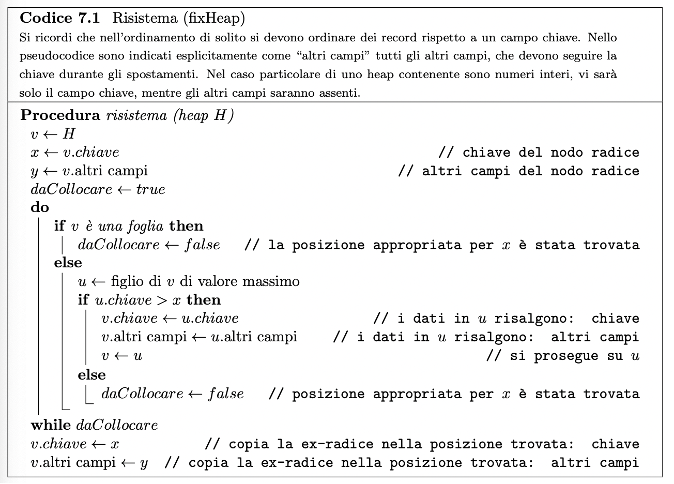
\includegraphics[scale=0.9]{risistemaheap}
\end{center}
\subsection*{Dato un albero binario quasi completo, come lo trasformo in uno heap?}
\begin{itemize}
\item con una tecnica divide-et-impera (top-down, ricorsiva)
\begin{center}
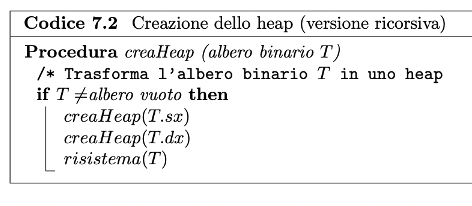
\includegraphics[scale=1]{creaheap1}
\end{center}
- se l'albero è vuoto, è già uno heap e non dobbiamo fare niente\\
- se l'albero non è vuoto, trasformo ricorsivamente in uno heap i due sottoalberi, e chiamo la procedura risistema, trasformando l'albero in uno heap
\item dai sottoalberi più piccoli a quelli più grandi (bottom-up, iterativa)
\begin{center}
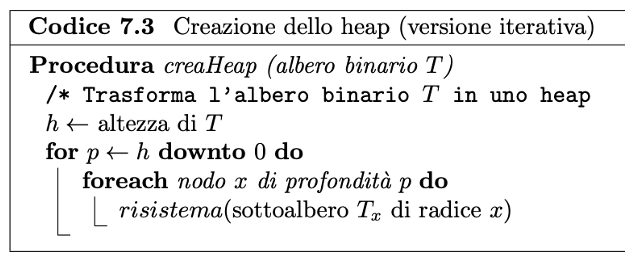
\includegraphics[scale=1]{creaheap2}
\end{center}
A partire dall'ultima foglia:\\
- considero ciascun nodo di profondità $h$ da destra a sinistra, trasformo in heap tutti i sottoalberi\\
- chiamo la procedura risistema\\
- ripeto sino ad arrivare alla radice
\end{itemize}
Abbiamo quindi tutti gli strumenti per finalmente implementare l'HeapSort

\section*{HeapSort}
HeapSort è un algoritmo iterativo basato sulla struttura dati chiamata heap. Questa struttura dati è rappresentabile con un array. L'heap è un albero binario quasi completo, in cui la chiave contenuta in ciascun nodo è maggiore o uguale al contenuto dei figli. Tutte le foglie si trovano all'ultimo o penultimo livello, e per ogni nodo, la chiave è $\geq$ delle chiavi nei figli.
\begin{center}
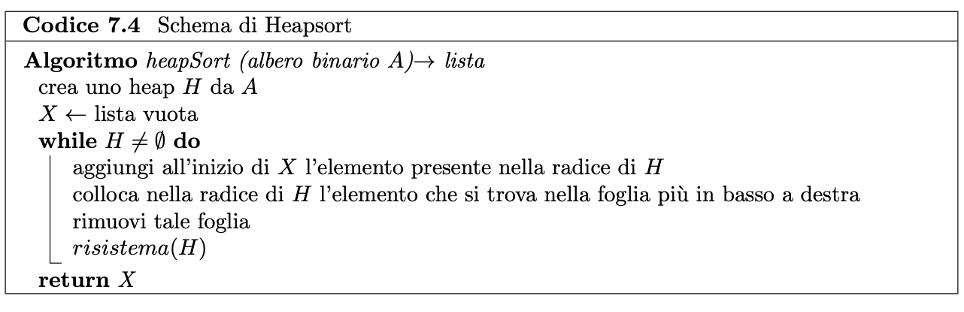
\includegraphics[scale=0.8]{heapsort}
\end{center}
Per funzionare l'HeapSort ha bisogno di una serie di metodi:\\
- risistema: che risistema un heap disordinato in un heap ordinato\\
- creaHeap: crea uno heap a partire da un albero binario\\\\
L'algoritmo di heapSort ha una complessità di \begin{center}
Per la \emph{parte esterna al while:} $T(n) = n$ \\
Per la \emph{parte interna al while:} $T(n) = nlogn$\\
Complessivamente: $O(nlogn)$
\end{center}
%\subsection{}



\end{document}  